%%%%%%%%%%%%%%%%%%%%%%%%%%%%%%%%%%%%%%%%%%%%%%%%%%%%%%%%%%%%%%%%%%%%%%
%%%%%%%%%%%%%%%%%%%%%%%%%%%%%%%%%%%%%%%%%%%%%%%%%%%%%%%%%%%%%%%%%%%%%%
%%
%% IVT LaTeX template
%%   Kirill M�ller
%%   kirill.mueller@ivt.baug.ethz.ch
%%
%%%%%%%%%%%%%%%%%%%%%%%%%%%%%%%%%%%%%%%%%%%%%%%%%%%%%%%%%%%%%%%%%%%%%%
%%%%%%%%%%%%%%%%%%%%%%%%%%%%%%%%%%%%%%%%%%%%%%%%%%%%%%%%%%%%%%%%%%%%%%

%%%%%%%%%%%%%%%%%%%%%%%%%%%%%%%%%%%%%%%%%%%%%%%%%%%%%%%%%%%%%%%%%%%%%%
%%%%%%%%%%%%%%%%%%%%%%%%%%%%%%%%%%%%%%%%%%%%%%%%%%%%%%%%%%%%%%%%%%%%%%
%%
%% Encoding check:
%%   �  �  �  �  �  �  �  �  �  �  �  �  �  �  �  �  �  �  �  �  �  �
%%
%%   If the above contains rubbish, please re-open this file using
%%   one of the following encodings: Latin1, ISO-8859-1, Windows-1252.
%%   DO NOT save the file in this case!
%%
%%%%%%%%%%%%%%%%%%%%%%%%%%%%%%%%%%%%%%%%%%%%%%%%%%%%%%%%%%%%%%%%%%%%%%
%%%%%%%%%%%%%%%%%%%%%%%%%%%%%%%%%%%%%%%%%%%%%%%%%%%%%%%%%%%%%%%%%%%%%%

%%%%%%%%%%%%%%%%%%%%%%%%%%%%%%%%%%%%%%%%%%%%%%%%%%%%%%%%%%%%%%%%%%%%%%
%%%%%%%%%%%%%%%%%%%%%%%%%%%%%%%%%%%%%%%%%%%%%%%%%%%%%%%%%%%%%%%%%%%%%%
%%
%% This is an example for writing a paper at the IVT.
%% It supports English and German language.
%% By using it, it is possible to switch paper layouts easily
%% (e.g., working paper style into TRB style)
%%
%% The easiest way to write you own paper is to create an
%% appropriate directory stucture in the papers subdirectory
%% i.e. papers/strc/2007/mypaper,
%% copy this template and modify it there.
%%
%% See the note below on renaming the main file.
%%
%% Each keyword is documented. Just follow the instructions...
%% Enjoy!
%%
%%%%%%%%%%%%%%%%%%%%%%%%%%%%%%%%%%%%%%%%%%%%%%%%%%%%%%%%%%%%%%%%%%%%%%
%%%%%%%%%%%%%%%%%%%%%%%%%%%%%%%%%%%%%%%%%%%%%%%%%%%%%%%%%%%%%%%%%%%%%%

%%%%%%%%%%%%%%%%%%%%%%%%%%%%%%%%%%%%%%%%%%%%%%%%%%%%%%%%%%%%%%%%%%%%%%
%%%%%%%%%%%%%%%%%%%%%%%%%%%%%%%%%%%%%%%%%%%%%%%%%%%%%%%%%%%%%%%%%%%%%%
%%
%% IMPORTANT NOTE ON FILE RENAMES:
%%   If you rename this file, look for the text "Template"
%%   in all files and change this to the new filename, too.
%%   In Linux/Mac OS X/Windows+cygwin: Execute the following command
%%     in the template directory (substitute NewName by the new
%%     base of the new file name):
%%
%%     find -maxdepth 1 -type f -exec sed -i 's/[T]emplate/NewName/g' \{\} \+
%%     mmv 'T''emplate.*' 'NewName.#1'
%%
%%   In Windows (vanilla): Use your favorite find-in-text-files tool
%%
%%%%%%%%%%%%%%%%%%%%%%%%%%%%%%%%%%%%%%%%%%%%%%%%%%%%%%%%%%%%%%%%%%%%%%
%%%%%%%%%%%%%%%%%%%%%%%%%%%%%%%%%%%%%%%%%%%%%%%%%%%%%%%%%%%%%%%%%%%%%%

%%%%%%%%%%%%%%%%%%%%%%%%%%%%%%%%%%%%%%%%%%%%%%%%%%%%%%%%%%%%%%%%%%%%%%
%% Location of the common files
%%   If unsure, please leave this as it is
\newcommand{\mypath}{_latexfiles/}
%\newcommand{\mypath}{../../../}
%%%%%%%%%%%%%%%%%%%%%%%%%%%%%%%%%%%%%%%%%%%%%%%%%%%%%%%%%%%%%%%%%%%%%%

%%%%%%%%%%%%%%%%%%%%%%%%%%%%%%%%%%%%%%%%%%%%%%%%%%%%%%%%%%%%%%%%%%%%%%
%% language specification:
%%   Here you define in which langugage your paper will be written.
%%   There are ALWAYS 2 languages to define (even you do not need it.)
%%   Since we are writing only in German or English, other languages
%%   are not supported.
%%   Choose either 'german' or 'english' as your first language.
\newcommand{\myfirstlang}{english}
%%%%%%%%%%%%%%%%%%%%%%%%%%%%%%%%%%%%%%%%%%%%%%%%%%%%%%%%%%%%%%%%%%%%%%

%%%%%%%%%%%%%%%%%%%%%%%%%%%%%%%%%%%%%%%%%%%%%%%%%%%%%%%%%%%%%%%%%%%%%%
%% Include Paper-Layout:
%%   Here the ivt working paper layout is chosen
%%   For changing this paper into i.e. TRB layout just change "ivt-wp"
%%   to "trb"
\input{\mypath_layouts/strc}
%%%%%%%%%%%%%%%%%%%%%%%%%%%%%%%%%%%%%%%%%%%%%%%%%%%%%%%%%%%%%%%%%%%%%%

%%%%%%%%%%%%%%%%%%%%%%%%%%%%%%%%%%%%%%%%%%%%%%%%%%%%%%%%%%%%%%%%%%%%%%
%%%%%%%%%%%%%%%%%%%%%%%%%%%%%%%%%%%%%%%%%%%%%%%%%%%%%%%%%%%%%%%%%%%%%%
%%
%% START DOCUMENT KEYWORDS
%%   In this part you can define Authors, Date, Titlefigure, etc...
%%
%%%%%%%%%%%%%%%%%%%%%%%%%%%%%%%%%%%%%%%%%%%%%%%%%%%%%%%%%%%%%%%%%%%%%%
%%%%%%%%%%%%%%%%%%%%%%%%%%%%%%%%%%%%%%%%%%%%%%%%%%%%%%%%%%%%%%%%%%%%%%

%%%%%%%%%%%%%%%%%%%%%%%%%%%%%%%%%%%%%%%%%%%%%%%%%%%%%%%%%%%%%%%%%%%%%%
%% The figure to include in the title page:
%% - {path/to/the/figure}: includes this figure in the title
%% - {}: no figure will be included
%% Note:
%%   do not write the ending of your figure ("MATSimLoop" instead
%%   of "MATSimLoop.pdf")
\newcommand{\mytitlefigure}{}
%%%%%%%%%%%%%%%%%%%%%%%%%%%%%%%%%%%%%%%%%%%%%%%%%%%%%%%%%%%%%%%%%%%%%%

%%%%%%%%%%%%%%%%%%%%%%%%%%%%%%%%%%%%%%%%%%%%%%%%%%%%%%%%%%%%%%%%%%%%%%
%% The title of the paper
\newcommand{\mytitle}{Estimating externalities from GPS traces using MATSim}
%%%%%%%%%%%%%%%%%%%%%%%%%%%%%%%%%%%%%%%%%%%%%%%%%%%%%%%%%%%%%%%%%%%%%%

%%%%%%%%%%%%%%%%%%%%%%%%%%%%%%%%%%%%%%%%%%%%%%%%%%%%%%%%%%%%%%%%%%%%%%
%% The institution (group) for which the paper is written
\newcommand{\myinstitutionDE}{}
\newcommand{\myinstitutionEN}{IVT ETHZ}
%%%%%%%%%%%%%%%%%%%%%%%%%%%%%%%%%%%%%%%%%%%%%%%%%%%%%%%%%%%%%%%%%%%%%%

%%%%%%%%%%%%%%%%%%%%%%%%%%%%%%%%%%%%%%%%%%%%%%%%%%%%%%%%%%%%%%%%%%%%%%
%% The number of the paper
\newcommand{\mynumber}{8XX}
%%%%%%%%%%%%%%%%%%%%%%%%%%%%%%%%%%%%%%%%%%%%%%%%%%%%%%%%%%%%%%%%%%%%%%

%%%%%%%%%%%%%%%%%%%%%%%%%%%%%%%%%%%%%%%%%%%%%%%%%%%%%%%%%%%%%%%%%%%%%%
%% The year of the paper
\newcommand{\myyear}{2018}
%%%%%%%%%%%%%%%%%%%%%%%%%%%%%%%%%%%%%%%%%%%%%%%%%%%%%%%%%%%%%%%%%%%%%%

%%%%%%%%%%%%%%%%%%%%%%%%%%%%%%%%%%%%%%%%%%%%%%%%%%%%%%%%%%%%%%%%%%%%%%
%% The month of the paper
%% - include only: jan,feb,mar,apr,may,jun,jul,aug,sep,oct,nov,dec
\newcommand{\mymonth}{may}
%%%%%%%%%%%%%%%%%%%%%%%%%%%%%%%%%%%%%%%%%%%%%%%%%%%%%%%%%%%%%%%%%%%%%%

%%%%%%%%%%%%%%%%%%%%%%%%%%%%%%%%%%%%%%%%%%%%%%%%%%%%%%%%%%%%%%%%%%%%%%
%% The day of the paper
%% - include day in number 1,..., 12,..., 31
\newcommand{\myday}{01}
%%%%%%%%%%%%%%%%%%%%%%%%%%%%%%%%%%%%%%%%%%%%%%%%%%%%%%%%%%%%%%%%%%%%%%

%%%%%%%%%%%%%%%%%%%%%%%%%%%%%%%%%%%%%%%%%%%%%%%%%%%%%%%%%%%%%%%%%%%%%%
%%
%% Define the authors
%% - if author name is left empty
%%   \newcommand{\mysecondauthor}{}
%%   it is not shown
%% - keep the right order (first, second, etc...) and keep the
%%   remaining entries empty!
%% - also add the way the authors appear in the reference style
%%
%%%%%%%%%%%%%%%%%%%%%%%%%%%%%%%%%%%%%%%%%%%%%%%%%%%%%%%%%%%%%%%%%%%%%%

%%%%%%%%%%%%%%%%%%%%%%%%%%%%%%%%%%%%%%%%%%%%%%%%%%%%%%%%%%%%%%%%%%%%%%
%% The author 1
\newcommand{\myfirstauthor}{Christopher Tchervenkov}
\newcommand{\myfirstauthorREF}{Tchervenkov,~C.}
%%%%%%%%%%%%%%%%%%%%%%%%%%%%%%%%%%%%%%%%%%%%%%%%%%%%%%%%%%%%%%%%%%%%%%
%% The author 2
\newcommand{\mysecondauthor}{Joseph Molloy}
\newcommand{\mysecondauthorREF}{Molloy,~J}
%%%%%%%%%%%%%%%%%%%%%%%%%%%%%%%%%%%%%%%%%%%%%%%%%%%%%%%%%%%%%%%%%%%%%%
%% The author 3
\newcommand{\mythirdauthor}{Kay W. Axhausen}
\newcommand{\mythirdauthorREF}{Axhausen,~K.W.}
%%%%%%%%%%%%%%%%%%%%%%%%%%%%%%%%%%%%%%%%%%%%%%%%%%%%%%%%%%%%%%%%%%%%%%
%% The author 4
\newcommand{\myfourthauthor}{}
\newcommand{\myfourthauthorREF}{}
%%%%%%%%%%%%%%%%%%%%%%%%%%%%%%%%%%%%%%%%%%%%%%%%%%%%%%%%%%%%%%%%%%%%%%
%% The author 5
\newcommand{\myfifthauthor}{}
\newcommand{\myfifthauthorREF}{}
%%%%%%%%%%%%%%%%%%%%%%%%%%%%%%%%%%%%%%%%%%%%%%%%%%%%%%%%%%%%%%%%%%%%%%
%% The author 6
\newcommand{\mysixthauthor}{}
\newcommand{\mysixthauthorREF}{}
%%%%%%%%%%%%%%%%%%%%%%%%%%%%%%%%%%%%%%%%%%%%%%%%%%%%%%%%%%%%%%%%%%%%%%
%% .. up to 12 authors supported by the templates
%%%%%%%%%%%%%%%%%%%%%%%%%%%%%%%%%%%%%%%%%%%%%%%%%%%%%%%%%%%%%%%%%%%%%%

%%%%%%%%%%%%%%%%%%%%%%%%%%%%%%%%%%%%%%%%%%%%%%%%%%%%%%%%%%%%%%%%%%%%%%
%%
%% Define the addresses
%% - if author name is left empty
%%   \newcommand{\mysecondaddress}{}
%%   it is not shown
%% - if two authors share the same affiliation, they should also use
%%   the same address
%% - keep the right order (first, second, etc...) and keep the
%%   remaining entries empty!
%% - also add the way the authors appear in the reference style
%%
%%%%%%%%%%%%%%%%%%%%%%%%%%%%%%%%%%%%%%%%%%%%%%%%%%%%%%%%%%%%%%%%%%%%%%

%%%%%%%%%%%%%%%%%%%%%%%%%%%%%%%%%%%%%%%%%%%%%%%%%%%%%%%%%%%%%%%%%%%%%%
%% Increase this if you have more than two addresses
\newcommand{\mynumaddresscolumns}{2}
%%%%%%%%%%%%%%%%%%%%%%%%%%%%%%%%%%%%%%%%%%%%%%%%%%%%%%%%%%%%%%%%%%%%%%
%% The first address
\newcommand{\myfirstaddress}{
  \createcontact{\myfirstauthor}%
  {IVT}
  {ETHZ}
  {CH-8093 Z�rich}
  {+41 44 633 33 17}
  {}
  {christopher.tchervenkov@ivt.baug.ethz.ch}
}
%%%%%%%%%%%%%%%%%%%%%%%%%%%%%%%%%%%%%%%%%%%%%%%%%%%%%%%%%%%%%%%%%%%%%%
%% The second address
\newcommand{\mysecondaddress}{
  \createcontact{\mysecondauthor}%
  {IVT}
  {ETHZ}
  {CH-8093 Z�rich}
  {+41 44 633 31 51}
  {}
  {joseph.molloy@ivt.baug.ethz.ch}
}
%%%%%%%%%%%%%%%%%%%%%%%%%%%%%%%%%%%%%%%%%%%%%%%%%%%%%%%%%%%%%%%%%%%%%%
%% The third address
\newcommand{\mythirdaddress}{
  \createcontact{\mythirdauthor}%
  {IVT}
  {ETHZ}
  {CH-8093 Z�rich}
  {+41 44 633 39 43}
  {}
  {axhausen@ivt.baug.ethz.ch}
}
%%%%%%%%%%%%%%%%%%%%%%%%%%%%%%%%%%%%%%%%%%%%%%%%%%%%%%%%%%%%%%%%%%%%%%
%% The fourth address
\newcommand{\myfourthaddress}{%
}
%%%%%%%%%%%%%%%%%%%%%%%%%%%%%%%%%%%%%%%%%%%%%%%%%%%%%%%%%%%%%%%%%%%%%%
%% The fifth address
\newcommand{\myfifthaddress}{%
}
%%%%%%%%%%%%%%%%%%%%%%%%%%%%%%%%%%%%%%%%%%%%%%%%%%%%%%%%%%%%%%%%%%%%%%
%% The sixth address
\newcommand{\mysixthaddress}{%
}

%%%%%%%%%%%%%%%%%%%%%%%%%%%%%%%%%%%%%%%%%%%%%%%%%%%%%%%%%%%%%%%%%%%%%%
%% The keywords (English)
\newcommand{\mykeywordsEN}{Keywords, in English, language}
%%%%%%%%%%%%%%%%%%%%%%%%%%%%%%%%%%%%%%%%%%%%%%%%%%%%%%%%%%%%%%%%%%%%%%

%%%%%%%%%%%%%%%%%%%%%%%%%%%%%%%%%%%%%%%%%%%%%%%%%%%%%%%%%%%%%%%%%%%%%%
%% The keywords (German)
\newcommand{\mykeywordsDE}{Schl�sselw�rter, auf Deutsch, Sprache}
%%%%%%%%%%%%%%%%%%%%%%%%%%%%%%%%%%%%%%%%%%%%%%%%%%%%%%%%%%%%%%%%%%%%%%

%%%%%%%%%%%%%%%%%%%%%%%%%%%%%%%%%%%%%%%%%%%%%%%%%%%%%%%%%%%%%%%%%%%%%%
%%%%%%%%%%%%%%%%%%%%%%%%%%%%%%%%%%%%%%%%%%%%%%%%%%%%%%%%%%%%%%%%%%%%%%
%%
%% END DOCUMENT KEYWORDS
%%
%%%%%%%%%%%%%%%%%%%%%%%%%%%%%%%%%%%%%%%%%%%%%%%%%%%%%%%%%%%%%%%%%%%%%%
%%%%%%%%%%%%%%%%%%%%%%%%%%%%%%%%%%%%%%%%%%%%%%%%%%%%%%%%%%%%%%%%%%%%%%


%%%%%%%%%%%%%%%%%%%%%%%%%%%%%%%%%%%%%%%%%%%%%%%%%%%%%%%%%%%%%%%%%%%%%%
%%%%%%%%%%%%%%%%%%%%%%%%%%%%%%%%%%%%%%%%%%%%%%%%%%%%%%%%%%%%%%%%%%%%%%
%%
%% START USER DEFINED COMMANDS
%%   Sometimes latex does not do hyphenations. This happens if it
%%   does not recognize a specific word. with "\hyphenation"
%%   you can add rules for those words
%% for advanced users:
%%   Advanced users can add additional commands here
%%
%%%%%%%%%%%%%%%%%%%%%%%%%%%%%%%%%%%%%%%%%%%%%%%%%%%%%%%%%%%%%%%%%%%%%%
%%%%%%%%%%%%%%%%%%%%%%%%%%%%%%%%%%%%%%%%%%%%%%%%%%%%%%%%%%%%%%%%%%%%%%

%%%%%%%%%%%%%%%%%%%%%%%%%%%%%%%%%%%%%%%%%%%%%%%%%%%%%%%%%%%%%%%%%%%%%%
%% Word split: unknown words for latex. show how to split them.
\hyphenation{Trenn-re-geln}
%%%%%%%%%%%%%%%%%%%%%%%%%%%%%%%%%%%%%%%%%%%%%%%%%%%%%%%%%%%%%%%%%%%%%%


%%%%%%%%%%%%%%%%%%%%%%%%%%%%%%%%%%%%%%%%%%%%%%%%%%%%%%%%%%%%%%%%%%%%%%
%%%%%%%%%%%%%%%%%%%%%%%%%%%%%%%%%%%%%%%%%%%%%%%%%%%%%%%%%%%%%%%%%%%%%%
%%
%% END USER DEFINED COMMANDS
%%
%%%%%%%%%%%%%%%%%%%%%%%%%%%%%%%%%%%%%%%%%%%%%%%%%%%%%%%%%%%%%%%%%%%%%%
%%%%%%%%%%%%%%%%%%%%%%%%%%%%%%%%%%%%%%%%%%%%%%%%%%%%%%%%%%%%%%%%%%%%%%

%%%%%%%%%%%%%%%%%%%%%%%%%%%%%%%%%%%%%%%%%%%%%%%%%%%%%%%%%%%%%%%%%%%%%%
%%%%%%%%%%%%%%%%%%%%%%%%%%%%%%%%%%%%%%%%%%%%%%%%%%%%%%%%%%%%%%%%%%%%%%
%%
%% To speed up compilation, you can split this file and move the
%%   contents of the upper part (just before the %&Template line)
%%   to a new file named Template.ltx.  This requires a working
%%   installation of GNU Make (included in Linux/Mac OS X,
%%   in Windows: through cygwin or GnuWin32).
%%
%&Template

%%%%%%%%%%%%%%%%%%%%%%%%%%%%%%%%%%%%%%%%%%%%%%%%%%%%%%%%%%%%%%%%%%%%%%
%%%%%%%%%%%%%%%%%%%%%%%%%%%%%%%%%%%%%%%%%%%%%%%%%%%%%%%%%%%%%%%%%%%%%%
%%
%% START OF DOCUMENT
%%   Here actually begins your document. The things below
%%   are a typical order in which a paper should be organized.
%%   Sometimes, editors have other suggestions. In this case
%%   just change the order in which each part should appear.
%%
%%%%%%%%%%%%%%%%%%%%%%%%%%%%%%%%%%%%%%%%%%%%%%%%%%%%%%%%%%%%%%%%%%%%%%
%%%%%%%%%%%%%%%%%%%%%%%%%%%%%%%%%%%%%%%%%%%%%%%%%%%%%%%%%%%%%%%%%%%%%%

\begin{document}

%%%%%%%%%%%%%%%%%%%%%%%%%%%%%%%%%%%%%%%%%%%%%%%%%%%%%%%%%%%%%%%%%%%%%%
%% Include the title page
\createtitlepage
%%%%%%%%%%%%%%%%%%%%%%%%%%%%%%%%%%%%%%%%%%%%%%%%%%%%%%%%%%%%%%%%%%%%%%

%%%%%%%%%%%%%%%%%%%%%%%%%%%%%%%%%%%%%%%%%%%%%%%%%%%%%%%%%%%%%%%%%%%%%%
%% Page numbering is taken care of by the templates
%%%%%%%%%%%%%%%%%%%%%%%%%%%%%%%%%%%%%%%%%%%%%%%%%%%%%%%%%%%%%%%%%%%%%%

%%%%%%%%%%%%%%%%%%%%%%%%%%%%%%%%%%%%%%%%%%%%%%%%%%%%%%%%%%%%%%%%%%%%%%
%% Table of contents
%\tableofcontents
%%%%%%%%%%%%%%%%%%%%%%%%%%%%%%%%%%%%%%%%%%%%%%%%%%%%%%%%%%%%%%%%%%%%%%

%%%%%%%%%%%%%%%%%%%%%%%%%%%%%%%%%%%%%%%%%%%%%%%%%%%%%%%%%%%%%%%%%%%%%%
%% List of figures and tables
%\listoffigures
%%%%%%%%%%%%%%%%%%%%%%%%%%%%%%%%%%%%%%%%%%%%%%%%%%%%%%%%%%%%%%%%%%%%%%

%%%%%%%%%%%%%%%%%%%%%%%%%%%%%%%%%%%%%%%%%%%%%%%%%%%%%%%%%%%%%%%%%%%%%%
%% List of tables
%\listoftables
%%%%%%%%%%%%%%%%%%%%%%%%%%%%%%%%%%%%%%%%%%%%%%%%%%%%%%%%%%%%%%%%%%%%%%

%%%%%%%%%%%%%%%%%%%%%%%%%%%%%%%%%%%%%%%%%%%%%%%%%%%%%%%%%%%%%%%%%%%%%%
%% If the next part should start at a new page insert \clearpage
%% command
\clearpage
%%%%%%%%%%%%%%%%%%%%%%%%%%%%%%%%%%%%%%%%%%%%%%%%%%%%%%%%%%%%%%%%%%%%%%

%%%%%%%%%%%%%%%%%%%%%%%%%%%%%%%%%%%%%%%%%%%%%%%%%%%%%%%%%%%%%%%%%%%%%%
%% Page numbering is taken care of by the templates
%%%%%%%%%%%%%%%%%%%%%%%%%%%%%%%%%%%%%%%%%%%%%%%%%%%%%%%%%%%%%%%%%%%%%%

%%%%%%%%%%%%%%%%%%%%%%%%%%%%%%%%%%%%%%%%%%%%%%%%%%%%%%%%%%%%%%%%%%%%%%

%%%%%%%%%%%%%%%%%%%%%%%%%%%%%%%%%%%%%%%%%%%%%%%%%%%%%%%%%%%%%%%%%%%%%%
%% ABSTRACT (first language)
%%   You can write it just here, if you want. You can also include
%%   an external .tex file (for better organization of you paper)
%%   The abstract MUST always be embedded into a command:
%%     \createabstract{
%%     This is an
%%     example abstract.
%%     }
%%   Be sure that your abstract is embedded into the curly brackets.
%%
%%   You can also put the abstract in a seperate .tex file for better
%%   organization. The command then is:
%%     \input{abstract-first}
%%   see also below (include sections)
\createabstract{
Providing people with information on the external costs of their mobility, including generated emissions, contribution to congestion, and noise pollution, has been shown to influence their travel behavior.
However, directly measuring these externalities at the source is unfeasible.
We have therefore developed a pipeline for estimating the generated externalities of recorded trips using the multi-agent simulation software MATSim. First, collected GPS traces are matched to the MATSim network and converted to MATSim events.
These events are then processed to impute externalities for each individual.
Emission values for various pollutants are calculated for each link using  the HBEFA database, accounting for vehicle type, road category and traffic conditions.
For congestion, we leverage MATSim modules developed by Kaddoura to compute average link delays for each hour of the day using the MATSim scenario of Switzerland, which are then assigned to links traveled by the participants.
We adapt this pipeline to further account for the Swiss valuation of externalities.
To validate our approach, the externalities generated for the Swiss MATSim scenario will be compared to ARE estimates and the swiss norm values.
The application of the pipeline will be demonstrated for GPS traces collected from the SBB Green Class project.
}

\section{Introduction}

It is increasingly recognized that both the environmental and social costs of travel need to be internalized to meet the demand on already strained transport networks by encouraging shifts in travel patterns. 
In this direction, there is a growing body of evidence that informal feedback on energy use can encourage more efficient behavior, both regarding home energy use \citep{faruqui2010impact} and travel behavior \citep{taniguchi2003psychological, fujii2006determinants}.
However, providing feedback on external costs in transport is particularly challenging, due to the heterogeneous nature of the users and privacy constraints.

%%Start here on externalities - Joe, already written
The main externalities of transportation can be divided into two groups: Those that affect other road users, namely congestion, and those that affect non-road users such as noise and emissions \cite{button2004rationale}.
The impact of congestion is primarily the loss of time spent waiting in traffic, where as emissions and noise have both environmental and health consequences.
When a person chooses to drive on a road, they only have to pay for the private time and car usage costs.
However, they do not have to pay the \textit{marginal social cost} (MSC) of their trip.
That is, the additional costs the driver imposes on other drivers by increasing demand on the route.
From economic theory, internalising this MSC in the form of a tax would reduce congestion and provide an overall social benefit \cite{arnott1994economics, pigou2013economics}). 

Micrsosimulation provides advantages from both the supply (network representation) and demand (individual agents) sides when modeling road pricing.
\citet{arnott2001economic} notes that traditional macroscopic models focus on link congestion, while ignoring or simplifying other elements of congestion such as nodal congestion, parking and interactions with pedestrians and spillback.
Microsimulated models allow for the representation of non-homogenous driver behaviour and preferences.
In particular, the importance of value of time heterogenity among individuals in road pricing models has been recognised by numerous researchers \citet{small2001value, verhoef2004product}.
Modern traffic microsimulation frameworks such as MATSim \cite{balmer2009matsim} are to capture range of externalities.

\citet{kaddoura2015marginal} developed an agent based marginal cost-pricing approaches for congestion, emissions and noise exteralities, and applied numerous models successfully to a large scale scenario of Greater Berlin.
When considering the internalisation of congestion costs, a particular contribution of his work, was to assign the external congestion costs to the causing agents.
In particular, \citet{kaddoura2015marginal} notes that it is simple to calculate the incurred congestion for each agent, but much more challenging to map it back to the causing agent.
The approach calculates each agent's contribution to the delays on traveled links using a queue based node-link model including spillback.

In real networks such an approach requires knowing the location and VTTS of every driver connected to a particular incident of congestion.
This is clearly unrealistic. Instead, this work presents an approach to impute externalities using just the GPS trace of the trip, a representation of the road network and aggregated congestion values generated from an agent-based MATSim simulation for Switzerland.

\subsection{Swiss MATSim Scenario}
%%Chris or Joe
The IVT 2015 Baseline Scenario \cite{boesch2015ivt} represents a typical working day in Switzerland for the year 2015.
As a MATSim scenario, the population consists of individual agents, each with daily travel plans (preferences), and social-demographic characteristics.
These agents represent the entire population of Switzerland on the network from \cite{boesch2015network}.
Of particular importance to this work, the 2015 scenario extends the work of \cite{Balmer2007switzerland} by including households and their incomes. 

\subsection{Swiss norms, ARE report, HBEFA}
%%Chris
The Swiss Federal Office of Spatial Development (ARE) published in 2016 an updated external costs and benefits analysis of transport in Switzerland \cite{are2016externalcosts}.
This analysis presents the most recent external costs and benefits calculations for the entire Swiss transport system, primarily focusing on external environmental, health and accident-related costs, utilizing the same methodology as \cite{ecoplaninfras2014externeeffekte}.
Specifically, external costs for 12 different cost categories are computed, differentiated by transport mode, type and user. 

\cite{foen2010pollutants} provides an updated detailed analysis of past and predicted future pollutant emissions due to road transport in Switzerland from 1990 to 2035.
The emission factors used in calculating these emissions are based on Version 3.1 of the Handbook for Emission Factor Analysis.
The HBEFA database contains emission factors for different vehicle categories and traffic situations, differentiated by emission type, pollutant and year.

An additional supplementary report on external traffic delay costs between 2010 and 2014 was published by MK Consulting and Infras in 2016 \cite{}.
\red{- how is 2013 data collected and results calculated?}
\red{- how are 2010-2014 values extrapolated?}
\red{Something about norms?}

\subsection{Green Class Data}
%%Joe
In the Green Class 2016 pilot project, the SBB created a new mobility offering for subscribers which consisted of a General Abonnenment (GA), an electric BMW i3, park+ride subscription, car and bike sharing subscriptions.
The 139 participants were tracked for the duration of the project using a mobile app enabled with GPS.
\red{how much detail on the work from geoINFK?} These GPS traces were processed to identify individual trips and modes of travel \cite{rabaul2016greenclassprocessing}.
A core component of the pilot project was the availability of an electric car to subscribers, powered by renewable energy.
Asumming similar driving behaviour independent of the drive-train type, the emissions avoided for each trip can calculated.
For this analysis, the dataset was filtered to include only trips with a start and finish within switzerland using either the electric car or personal automobile. 

\section{Methodology}
%% i.e. Pipeline structure
%%Joe

\section{Results}
%% i.e. validation against swiss norms
\subsection{Validation}
%%Chris
To validate the externality values estimated using MATSim, the produced outputs are analyzed both temporally and spatially to check for plausibility and then compared with the estimations from previous Swiss external cost reports.

\subsubsection{Emissions}
Emissions values can be estimated with MATSim directly from the processed GPS traces and therefore do not explicitely require a calibrated MATSim scenario for Switzerland.
Nevertheless, in order to validate our estimation, emission values are first calculated using a 10\% MATSim scenario for Switzerland.
To comply with new vehicle registrations statistics according to \cite{autoschweiz2010} and \cite{autoschweiz2012} as well as the vehicle ownership predictions from \cite{foen2010pollutants}, two scenarios where 30\% and 40\% of vehicles are assigned a diesel engine were examined.

The emission values are estimated for each road link in the MATSim network for the following pollutants: CO, CO$_2$(total), FC, HC, NMHC, NO$_2$, NO$_x$, PM and SO$_2$.
The values are aggregated into hourly time bins.
These emission estimates are then first analyzed temporally and spatially to assure the plausibility of the output.

When analyzing the temporal evolution of emissions over the course of a typical workday, we would expect it to correlate with typical commuter patterns, i.e. low emissions both in the early morning and late evening and higher emissions during the day, with spikes corresponding to rush-hour periods.
\Cref{fig:hourlyEmissions} shows the typical daily emission of each pollutant per hourly time bin estimated from the MATSim scenario, for both the 30\% and 40\% diesel engine ownership scenarios.
Note that only total CO$_2$ and FC are shown, as the emissions values for the other pollutants are negligeable in comparison.
As expected, two distinct peaks corresponding to morning and evening rush-hours can be observed, while the early morning and late-night values are near zero and the midday values lie somewhere in between.

\createfigure%
{Hourly emissions values for Switzerland}%
{Hourly emissions values for Switzerland. Only CO$_2$ and FC emissions are shown, as the values for the other pollutants are negligeable in comparison.}%
{\label{fig:hourlyEmissions}}%
{%
  \createsubfigure%
  {30\% diesel vehicles}%
  {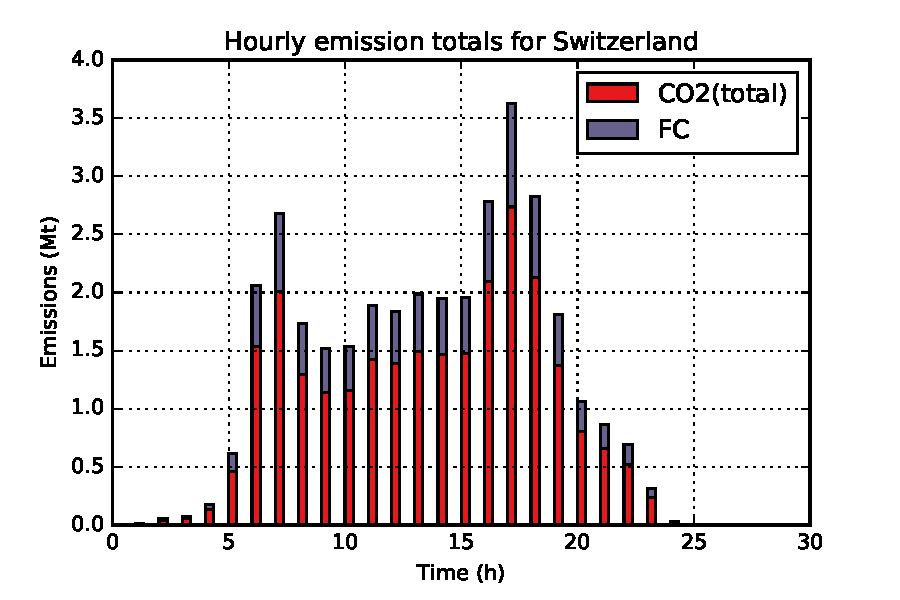
\includegraphics[width=0.49\textwidth,
angle=0]{figures/hourly_emissions_30pct_diesel.pdf}}%
  {\label{fig:hourlyEmissions-30pctDiesel}}%
  {}%
  \createsubfigure%
  {40\% diesel vehicles}%
  {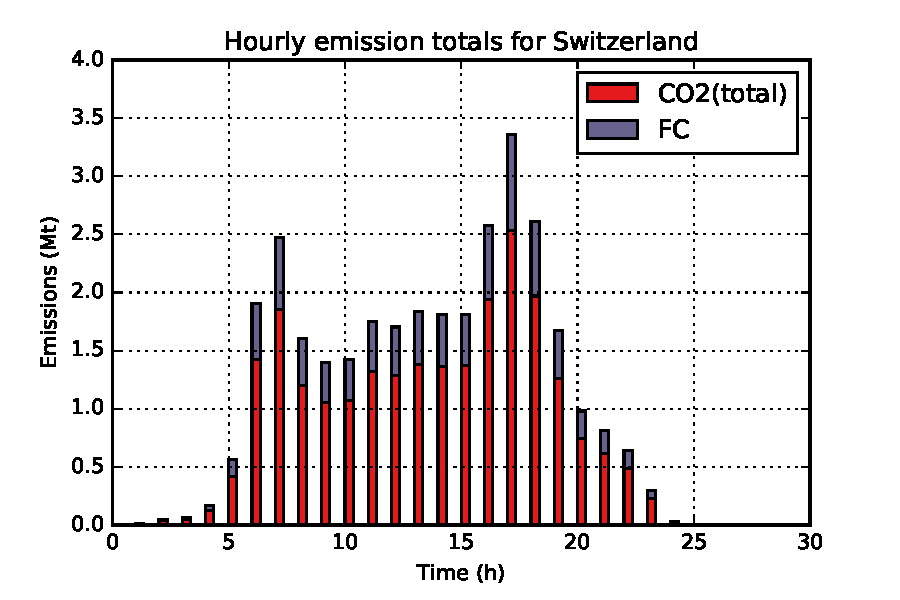
\includegraphics[width=0.49\textwidth,
angle=0]{figures/hourly_emissions_40pct_diesel.pdf}}%
  {\label{fig:hourlyEmissions-30pctDiesel}}%
  {}%
}%
{}

The spatial analysis of emissions is expected to show higher emissions in and around larger cities and within highly populated cantons, where more people live and therefore more commutes are observed.
Fig. shows the spatial distribution of the total daily emissions over entire Switzerland whereas Fig. show aggregated total daily emissions per canton.
Indeed, it can be seen that larger cities such as Zurich and Bern and highly populated canton such as Zurich, Bern and Vaud produce higher total emissions than rural areas within e.g. Graub�nden, Schwyz or Appenzell.

\createfigure%
{Spatial distribution of total emissions in Switzerland}%
{Spatial distribution of total emissions in Switzerland}%
{\label{fig:spatialEmissions}}%
{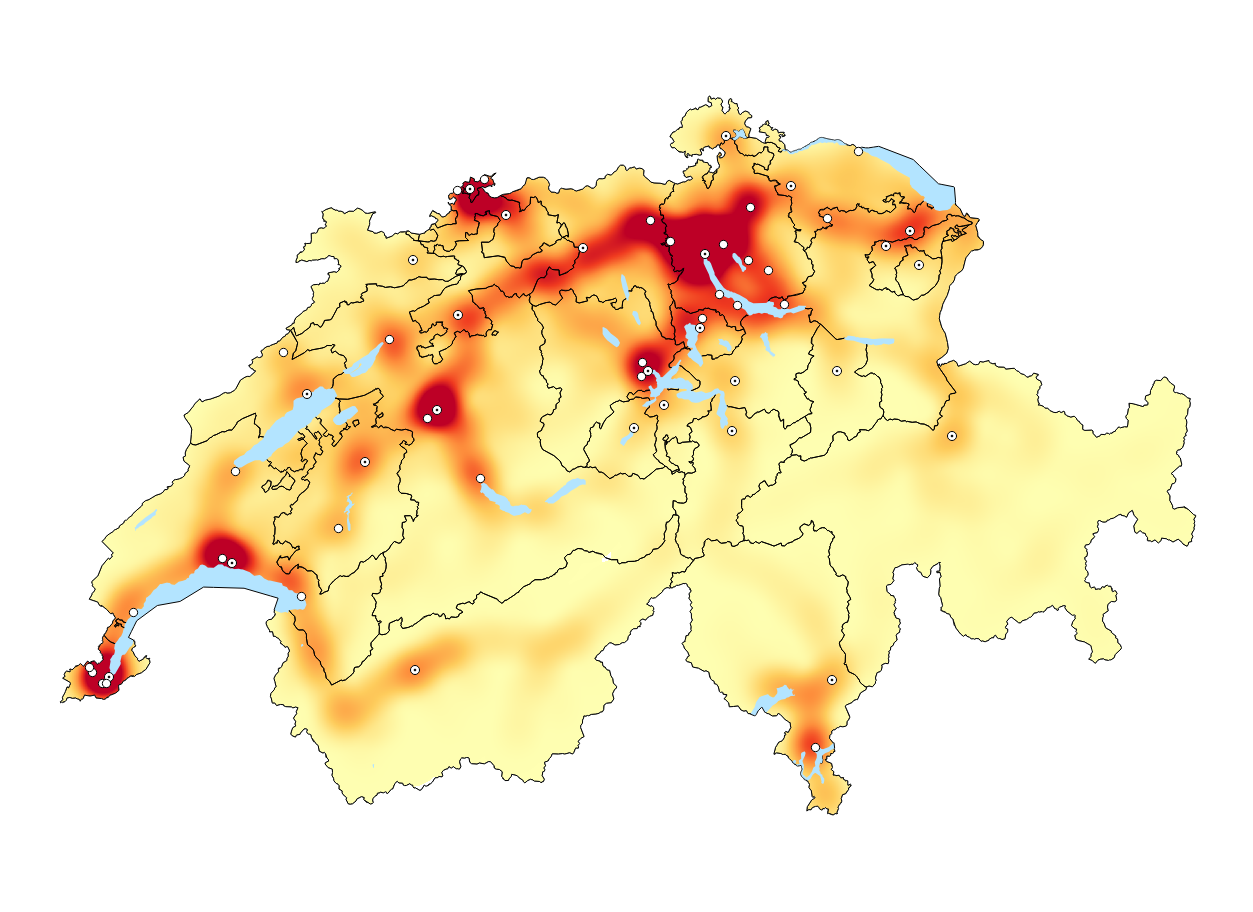
\includegraphics[width=1.0\textwidth, angle=0]{figures/total_emissions_heatmap.png}}%
{}

The MATSim computed emissions values are then compared to those calculated by \cite{foen2010pollutants} for 2015.
Since MATSim simulates a single typical workday for 10\% of the entire Swiss population, our values need to be scaled in order to be comparable.
The emissions values are thus multiplied by 10 to account for the population sampling, then by 365 days and finally by an additional scale factor such that the total traveled distance matches the one reported by \cite{foen2010pollutants} for 2015.
\Cref{tab:emissionValueMatsimFoenComparison} shows the total estimated emissions values for both MATSim scenarios and \cite{foen2010pollutants} and \Cref{fig:emissionValueMatsimFoenComparison} plots the percent deviation of the MATSim estimates from the reported 2015 estimates.
The total emission values for all pollutants except PM are within 20\% of the reported values with 30\% diesel engine ownership; they lie within 10\% in the 40\% diesel engine ownership case.
These deviations are possibly due to the fact that emissions factors depend on the exact type of petrol or diesel engine.
In the MATSim model, only one type of petrol and diesel engine is considered, whereas in reality, these are further subdivided into specific subtypes.
Nevertheless, the estimed values are coincide with the previously reported values, thereby demonstrating that MATSim provides a reliable means of estimating emission values for pollutants.

\createtable%
{MATSim and FOEN estimated emission value comparison}%
{MATSim and FOEN estimated emission value comparison}%
{\label{tab:emissionValueMatsimFoenComparison}}%
{%
  \begin{tabular}[c]{lrrrrr}
    \toprule
    \multirow{3}{*}{Pollutant} & \multirow{3}{*}{FOEN} & \multicolumn{4}{c}{MATSim} \\ 
    & & \multicolumn{2}{c}{30\% diesel} & \multicolumn{2}{c}{40\% diesel}\\
    & g & g & \% & g & \% \\
    \midrule
    CO$_2$(total) & 10687911 & 11770667 &  10.13 & 10893138 &   1.92 \\
    FC &                  NA &  3872146 &    --- &  3582233 &    --- \\
    CO &               67424 &    69526 &   3.12 &    61283 &  -9.11 \\
    NOx &              16496 &    14004 & -15.11 &    17220 &   4.39 \\
    HC &                9546 &     9820 &   2.87 &     8777 &  -8.06 \\
    NMHC &              9037 &     9291 &   2.81 &     8315 &  -7.98 \\
    NO2 &               4127 &     3410 & -17.38 &     4471 &   8.34 \\
    PM &                 418 &      523 &  25.16 &      672 &  60.85 \\
    SO2 &                 59 &       57 &  -3.56 &       53 & -10.48 \\
    \bottomrule
  \end{tabular}
}%
{}

\createfigure%
{MATSim and FOEN estimated emission value comparison}%
{MATSim and FOEN estimated emission value comparison}%
{\label{fig:emissionValueMatsimFoenComparison}}%
{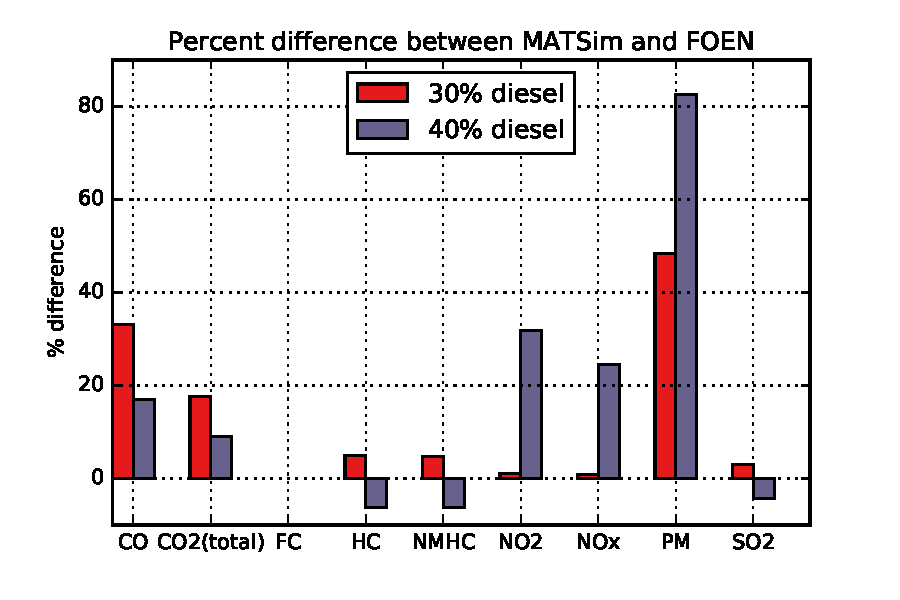
\includegraphics[width=1.0\textwidth, angle=0]{figures/percent_differences.pdf}}%
{}

\subsubsection{Congestion}

Contrary to emissions, congestion and delays caused to others cannot directly be estimated from GPS traces alone, since information on how many other drivers were present on the road at that given moment is lacking.
It is precisely for this reason that MATSim is used to estimate congestion throughout a typical workday.
Therefore, it is crucial that the estimated aggregate congestion values are consistent with other previous estimates.
As before, these values are calculated using a 10\% MATSim scenario for Switzerland and are aggregated into hourly time bins per road link.
These estimates are again first analyzed temporally and spatially to assure the plausibility of the output before being compared to \cite{} \red{citation}.

The typical total caused delays pattern per hourly time bin estimated from the MATSim scenario is shown in \Cref{fig:hourlyDelays}.
As was the case for emissions, total delays also expectedly coincide with typical commuter patterns, with fewer delays the early morning and at night, two distinct peaks corresponding to morning and evening rush-hours and midrange values at midday.

\createfigure%
{Hourly total caused delays for Switzerland}%
{Hourly total caused delays for Switzerland}%
{\label{fig:hourlyDelays}}%
{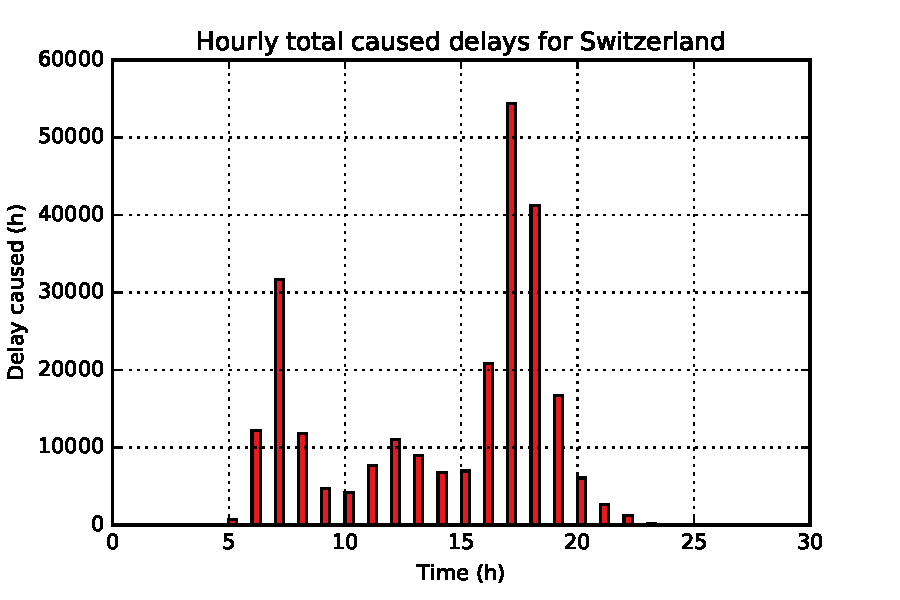
\includegraphics[width=0.49\textwidth,
angle=0]{figures/hourly_caused_delays.pdf}}%
{}

\Cref{fig:hourlyDelays} shows the spatial distribution of the total daily caused delays over entire Switzerland.
Following an anogolous reasoning as for emissions, longer delay times are observed in and around larger cities and within highly populated cantons, where more people live and commute to.

\createfigure%
{Spatial distribution of total emissions in Switzerland}%
{Spatial distribution of total emissions in Switzerland}%
{\label{fig:spatialDelays}}%
{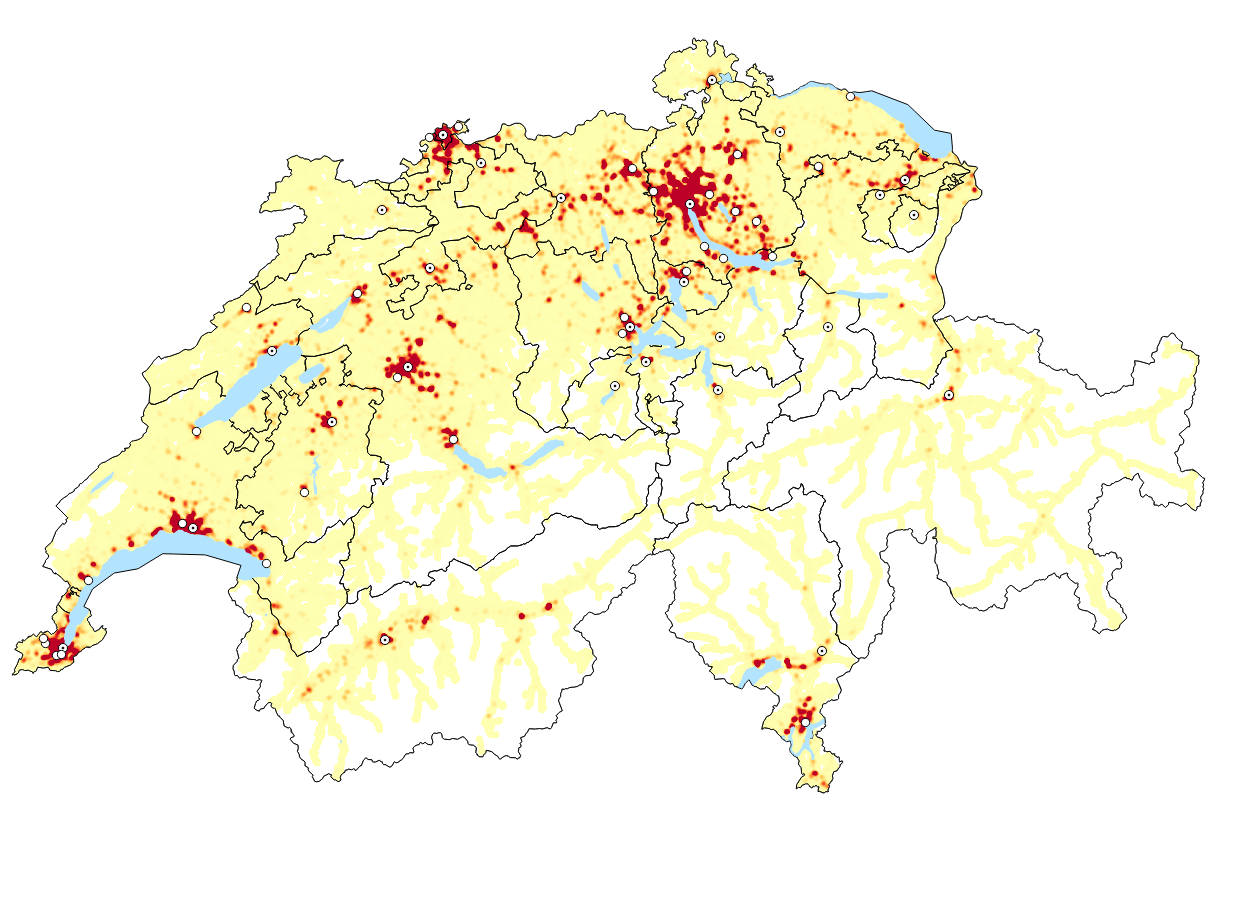
\includegraphics[width=1.0\textwidth, angle=0]{figures/delays_heatmap.png}}%
{}

The MATSim computed emissions values are then compared to those calculated by \cite{}.
The same scaling operations are performed as in the case of emissions: multiplication by 10 to account for the population sampling, then by 365 days and finally by an additional scale factor such that the total traveled distance matches the one reported by \cite{foen2010pollutants} for 2015.


\subsection{Green Class Emission Reductions}
%%Joe
\section{Conclusion}
%%Chris


%%%%%%%%%%%%%%%%%%%%%%%%%%%%%%%%%%%%%%%%%%%%%%%%%%%%%%%%%%%%%%%%%%%%%%
%% Bibliography
%%   Leave this as is, and add you own entries to my.bib
%%   Many references are already defined in _latexfiles/bibs/all-eng.bib
%%   Refer to the BibTeX/LaTeX tutorial for adding new entries
%%   to the IVT BibTeX database
\bibliography{\mypath bibs/all-eng,my}
%%%%%%%%%%%%%%%%%%%%%%%%%%%%%%%%%%%%%%%%%%%%%%%%%%%%%%%%%%%%%%%%%%%%%%

%%%%%%%%%%%%%%%%%%%%%%%%%%%%%%%%%%%%%%%%%%%%%%%%%%%%%%%%%%%%%%%%%%%%%%
%% Appendices
%%   Usually they would start on a separate page
%%%%%%%%%%%%%%%%%%%%%%%%%%%%%%%%%%%%%%%%%%%%%%%%%%%%%%%%%%%%%%%%%%%%%%

\clearpage
\appendix

%%%%%%%%%%%%%%%%%%%%%%%%%%%%%%%%%%%%%%%%%%%%%%%%%%%%%%%%%%%%%%%%%%%%%%
%
\section{First section in the appendix} \label{sec:a1}
%
%%%%%%%%%%%%%%%%%%%%%%%%%%%%%%%%%%%%%%%%%%%%%%%%%%%%%%%%%%%%%%%%%%%%%%

The appendix starts with the ``appendix'' command. the rest is the same as in the sections.

%%%%%%%%%%%%%%%%%%%%%%%%%%%%%%%%%%%%%%%%%%%%%%%%%%%%%%%%%%%%%%%%%%%%%%
\subsection{A subsection in the appendix} \label{sec:a1-subsection}
%%%%%%%%%%%%%%%%%%%%%%%%%%%%%%%%%%%%%%%%%%%%%%%%%%%%%%%%%%%%%%%%%%%%%%

bla bla bla bla bla bla bla bla bla bla bla bla bla bla bla bla bla bla bla bla bla bla bla bla bla bla bla bla bla bla bla bla bla bla bla bla bla bla

bla bla bla bla bla bla bla bla bla bla bla bla
bla bla bla bla bla bla bla bla bla bla bla bla bla bla bla bla bla bla bla bla bla bla bla bla bla bla bla bla bla bla bla bla bla bla bla bla bla bla bla bla bla bla bla bla bla bla bla bla bla bla bla bla bla bla bla bla bla bla bla bla bla bla bla bla bla bla bla bla bla bla bla bla bla bla bla bla bla bla bla bla bla bla bla bla bla bla bla bla bla bla bla bla bla bla bla bla bla bla bla bla
bla bla bla bla bla bla bla bla bla bla bla bla bla bla bla bla bla bla bla bla bla bla bla bla bla bla bla bla bla bla bla bla bla bla bla bla bla bla bla bla

%%%%%%%%%%%%%%%%%%%%%%%%%%%%%%%%%%%%%%%%%%%%%%%%%%%%%%%%%%%%
\section{Second section in the appendix}
%%%%%%%%%%%%%%%%%%%%%%%%%%%%%%%%%%%%%%%%%%%%%%%%%%%%%%%%%%%%

bla bla bla bla bla bla bla bla bla bla bla bla
bla bla bla bla bla bla bla bla bla bla bla bla bla bla bla bla bla bla bla bla bla bla bla bla bla bla bla bla bla bla bla bla bla bla bla bla bla bla bla bla bla bla bla bla bla bla bla bla bla bla bla bla bla bla bla bla bla bla bla bla bla bla bla bla bla bla bla bla bla bla bla bla bla bla bla bla bla bla bla bla bla bla bla bla bla bla bla bla bla bla bla bla bla bla bla bla bla bla bla bla
bla bla bla bla bla bla bla bla bla bla bla bla bla bla bla bla bla bla bla bla bla bla bla bla bla bla bla bla bla bla bla bla bla bla bla bla bla bla bla bla


\end{document}

%%%%%%%%%%%%%%%%%%%%%%%%%%%%%%%%%%%%%%%%%%%%%%%%%%%%%%%%%%%%%%%%%%%%%%
%%%%%%%%%%%%%%%%%%%%%%%%%%%%%%%%%%%%%%%%%%%%%%%%%%%%%%%%%%%%%%%%%%%%%%
%%
%% END OF DOCUMENT
%%
%%%%%%%%%%%%%%%%%%%%%%%%%%%%%%%%%%%%%%%%%%%%%%%%%%%%%%%%%%%%%%%%%%%%%%
%%%%%%%%%%%%%%%%%%%%%%%%%%%%%%%%%%%%%%%%%%%%%%%%%%%%%%%%%%%%%%%%%%%%%%

%%%%%%%%%%%%%%%%%%%%%%%%%%%%%%%%%%%%%%%%%%%%%%%%%%%%%%%%%%%%%%%%%%%%%%
%% Editor specific keywords:
%%   This is not part of you paper, but sometimes it is used
%%   for additional features of TeX Editors.
%%
%% WinEdt:
%%   to get the bibliography list
%GATHER{./_bibs/all-eng.bib}
